\documentclass[main.tex]{subfiles}

\begin{document}

\section{Aufgabe 4}
Gegeben sei die Funktion
\begin{equation*}
    f(x) =x^{4} -5x^{2} + 4
\end{equation*}

\begin{enumerate}
    \item[(a)] Beweisen Sie, dass $f(x)$ mindestens eine Nullstelle im Intervall $\left[ -\frac{3}{2} ;\frac{1}{2}\right]$ besitzt.
    \item[(b)] Welche Auswirkung hat die Vergrößerung des zu untersuchenden Intervall auf $\left[ -\frac{5}{2} ;\frac{1}{2}\right]$? Was bedeutet dies für die Nullstellensuche?
    \item[(c)] Wie viele Nullstellen kann ein Polynom $n$-ten Gerades maximal haben?
\end{enumerate}

\subsection{Lösung 4}

\begin{figure}[ht]
	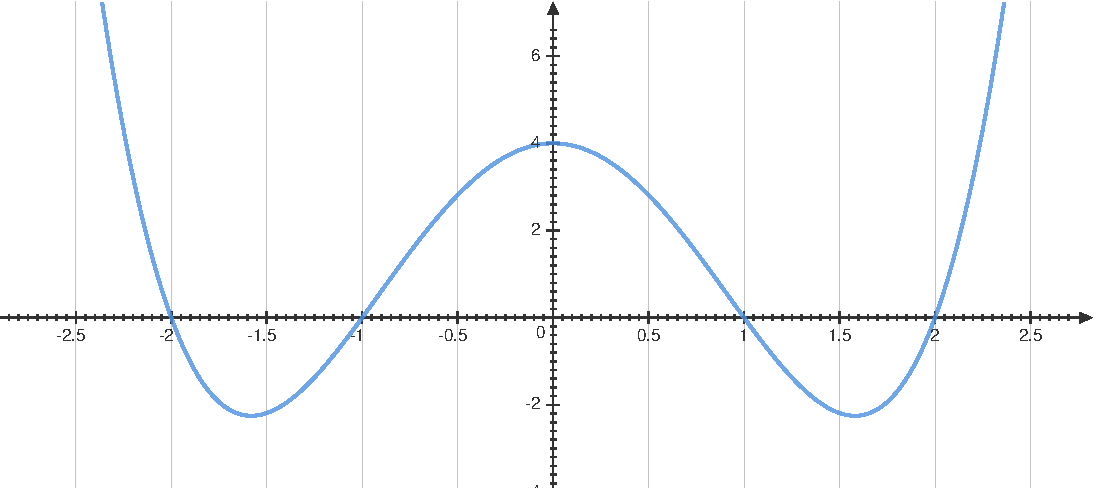
\includegraphics[width=\linewidth]{fig-4a.pdf}
	\caption{Graph von $f(x)$}
\end{figure}

\subsubsection{Lösung 4a}
Untersuchung mit Nullstellensatz (die Stetigkeit des Polynoms kann vorausgesetzt werden):
\begin{gather*}
    f\left( -\frac{3}{2}\right) =-\frac{35}{16} \ \text{und} \ f\left(\frac{1}{2}\right) =\frac{45}{16}\\
    \\
    f\left( -\frac{3}{2}\right) \cdot f\left(\frac{1}{2}\right) < 0\Longrightarrow \exists \ x^{*} \in \left[ -\frac{3}{2} ;\frac{1}{2}\right] \ \text{mit} \ f\left( x^{*}\right) =0
\end{gather*}

\subsubsection{Lösung 4b}
Die Untersuchung mit dem Nullstellensatz funktioniert nun nicht mehr, da mit
\begin{gather*}
    f\left( -\frac{5}{2}\right) =\frac{189}{16}\\
    \\
    f\left( -\frac{5}{2}\right) \cdot f\left(\frac{1}{2}\right)  >0\nRightarrow \exists \ x^{*} \in \left[ -\frac{5}{2} ;\frac{1}{2}\right] \ \text{mit} \ f\left( x^{*}\right) =0
\end{gather*}
keine oder eine gerade Anzahl an Nullstellen vorliegen können.

\subsubsection{Lösung 4c}
Ein Polynom $p$ vom Grad $n$ kann keine oder endlich viele, aber maximal $n$ verschiedene Nullstellen haben $x_1,x_2,\ldots, x_r\ (r \leq n)$.


\end{document}
